\documentclass[a4paper,10pt]{scrartcl}
\usepackage{hyperref}
\hypersetup{
    unicode=false,          % non-Latin characters in Acrobat’s bookmarks
    pdftoolbar=true,        % show Acrobat’s toolbar?
    pdfmenubar=true,        % show Acrobat’s menu?
    pdffitwindow=false,     % window fit to page when opened
    pdfstartview={FitH},    % fits the width of the page to the window
    pdftitle={TNC@FHH documentation version 0.7.0},    % title
    pdfauthor={Author},     % author
    pdfsubject={Subject},   % subject of the document
    pdfcreator={Creator},   % creator of the document
    pdfproducer={Producer}, % producer of the document
    pdfkeywords={keywords}, % list of keywords
    pdfnewwindow=true,      % links in new window
    colorlinks=true,        % false: boxed links; true: colored links
    linkcolor=blue,          % color of internal links
    citecolor=green,        % color of links to bibliography
    filecolor=magenta,      % color of file links
    urlcolor=blue           % color of external links
}

\usepackage{graphicx}

\usepackage{listings,color}   %% color für Farbmarkierungen
\definecolor{LightBlue}{rgb}{0.9, 0.9, 1.0}
\definecolor{LightRed}{rgb}{1.0, 0.9, 0.8}
\definecolor{LightGreen}{rgb}{0.1, 0.7, 0.1}
\lstset{ basicstyle=\ttfamily\scriptsize,%\scriptsize,
		keywordstyle=\color{blue},
		identifierstyle=\bfseries,
        commentstyle=\color{LightGreen},
		language=C++,
		frame=none,
		showstringspaces=false,
		backgroundcolor=\color{LightBlue},
        breaklines=true}

% listings for freeradius-eapttls-config files
\lstdefinestyle{eapttls-config}{language=sh, % Sprache = sh
	basicstyle=\ttfamily\scriptsize,%\scriptsize,
	keywordstyle=\color{blue},
	commentstyle=\color{LightGreen},
	stringstyle=\color{red},
	breaklines=true,
	keepspaces=true,
	showstringspaces=false,
	frame=none,
	backgroundcolor=\color{LightBlue}}

% newcommand \code{}

\newcommand{\code}[1]{{\tt{#1}}}

% newcommands for freeradius-eapttls-patch files
\newcommand{\radd}[1]{\texttt{#1}}	% for debug-output
\newcommand{\radf}[1]{\textsc{#1}} % for files
\newcommand{\radm}[1]{\textsl{#1}} % for methods

%opening

\begin{document}
\titlehead{
\begin{minipage}{0.55\textwidth}
  {\Large Fachhochschule Hannover\\}
  University of Applied Sciences and Arts\\
  Faculty IV - Department of Computer Science\\
  Trust@FHH Research Group\\
  \url{http://trust.inform.fh-hannover.de}\\
  \href{mailto:trust@f4-i.fh-hannover.de}{trust@f4-i.fh-hannover.de}
\end{minipage}
\begin{minipage}{0.45\textwidth}
  \hfill
  \includegraphics[width=0.9\textwidth,height=!]{figures/logo-trustfhh.pdf}
\end{minipage}
}
\subject{Documentation Version 0.7.0}
\title{TNC@FHH \\~\\ An Open Source TNC Implementation}
%\subtitle{Klein aber fein?} % geht nicht unter ubuntu 9.10 texlive version
\author{Ingo Bente, Bastian Hellmann, Jan Bernhardt, Arne Welzel}
\date{\today}
\publishers{Trust@FHH Research Group}

\maketitle

\tableofcontents

\begin{abstract}
This documentation describes the TNC@FHH software version 0.7.0. It covers all
subprojects of TNC@FHH and highlights the overall project structure. Furthermore,
it gives examples how to use parts of the TNC@FHH framework in your own projects (like
coding your own IMC/V based upon TNC@FHH). This document is (although contained in
this release) still a work in progress. We try to keep it up to date, but some sections might refer to older versions of TNC@FHH\footnote{E.g., some of the UML diagrams refer to version 0.6.0 since there were no substantial changes.}. Please report any issues related to it to
\href{mailto:trust@f4-i.fh-hannover.de}{trust@f4-i.fh-hannover.de}. This document
does \emph{not} describe all configuration options and tasks in order to set up
a TNC@FHH environment. For installation and configuration issues, please
refer to the README file and to our wiki: \url{http://trust.inform.fh-hannover.de/wiki}.
\end{abstract}

% ==============================================================================
\section{Introduction}
The TNC@FHH project is an open source implementation of the Trusted Network
Connect (TNC) framework which is specified by the Trusted Computing Group
(TCG). TNC@FHH allows you to provision access to a network based upon
factors like the user credentials and the requesting endpoint's integrity state.

The following TNC components and their respective interfaces are implemented by
TNC@FHH:
\begin{itemize}
	\item IMCs (IF-IMC 1.2)
	\item IMVs (IF-IMV 1.2)
	\item TNCS (IF-TNCCS 1.1)
	\item NAA  (IF-T EAP 1.1)
\end{itemize}

On the Policy Decision Point, TNC@FHH works as an extension to FreeRADIUS.
FreeRADIUS handles the user authentication and all of the standard EAP message
processing. TNC@FHH is plugged into FreeRADIUS via a new EAP module that
supports TNC.

\section{Project Structure}
TNC@FHH consists of several subprojects:
\begin{description}
    \item[freeradius-eaptnc-patch] Patch for FreeRADIUS to add support for TNC. This is basically a new EAP
    module that handles the TNC traffic and forwards the TNC specific data to the
    naaeap module. The patch is implemented in C.
     \item[freeradius-eapttls-patch] Patch for FreeRADIUS to add support for multiple EAP-methods to be tunneld within one EAP-TTLS channel. This explicitly supports
     to chain multiple EAP methods, i.e. EAP-MD5 (for user authentication) and then EAP-TNC (for endpoint assessment) in one EAP-TTLS tunnel.
     The patch is implemented in C.
    \item[naaeap] A shared library that is used by the EAP TNC module. It parses the EAP-TNC data,
    handles fragmentation and forwards the parsed data (i.e. a TNCCS message) to the tncs module.
    Outgoing TNCCS messages are in turn properly encapsulated within EAP TNC.
    naaeap is implemented in C++.
    \item[tncs] tncs is a shared library that is used by the naaeap module. It represents the
    TNCS component within the TNC architecture. tncs handles the communication with the IMVs that are installed on the PDP and the TNCC on the AR. tncs is implemented in C++.
    \item[imunit] imunit is a framework for developing IMC/V pairs. All TNC@FHH IMC/V pairs are
    based upon imunit. imunit is implemented in C++.
    \item[IMC/V pairs] TNC@FHH comes with a set of working IMC/V pairs:
    \begin{itemize}
    	\item example: A hello world example of an imc/v pair.
    	\item dummy: Another hello world example with a bit more functionality.
    	\item clamav: Checks the status of the AV software clamav.
    	\item platid: Allows to authenticate an endpoint based upon X.509 certificates (supports
        TPMs)
    	\item attestation: Allows to verify the integrity of an endpoint based on TPM attestation (using AIKs).
        \item hostscanner: Allows to check the status of arbitrary ports on an endpoint.
    \end{itemize}
    \item[tncsim] This is a simple test program that acts both as TNCC and TNCS,
    but without an NAR or NAA component. It was developed to ease the testing of
    IMC/V pairs. It uses libtnc as client and TNC@FHH tncs as server. tncsim can
    load both IMCs and IMVs and starts a single TNC handshake by calling
    \texttt{beginHandhake()} for each IMC. tncsim is implemented in C++.
\end{description}

Figure \ref{fig:tncfhh-project-structure} gives an overview of the existing subprojects and der dependencies.
\begin{figure}
 \centering
   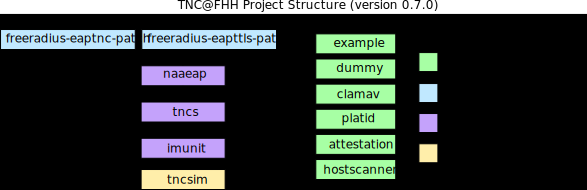
\includegraphics[width=\textwidth,height=!]{figures/tncfhh-project-structure-0-7-0.pdf}
 \caption{Project Structure of TNC@FHH}
 \label{fig:tncfhh-project-structure}
\end{figure}

Detailed information about each subproject is given in the following sections.

% ==============================================================================
\section{Building and Installing TNC@FHH}
Since version 0.7.0, there is only one TNC@FHH tarball available that contains all
software components. This makes the build and install process a lot easier. The
following prerequisites should be fulfilled in order to be able to build all TNC@FHH components:
\begin{itemize}
    \item cmake\\
	(use the version provided by your distribution)
    \item log4cxx (mandatory for all components)\\
	(use the version provided by your distribution)
	\item xerces-c (needed by tncs)\\
	(use the version provided by your distribution)
	\item trousers $>=$ 0.3.4 (needed by attestation IMC)\\ \url{http://sourceforge.net/projects/trousers/}
	\item libtnc $>=$ 1.24 (needed by tncsim)\\ \url{http://sourceforge.net/projects/libtnc/}
\end{itemize}

To build (and optionally install) TNC@FHH with its default configuration, just do the following:

\begin{lstlisting}
// extract archive
tar -xzf tncfhh-0.7.0.tar.gz
// switch to directory
cd tncfhh-0.7.0
// create build directory
mkdir build
// switch to build directory
cd build
// build (and optionally install) TNC@FHH
cmake ../
make
make install
\end{lstlisting}

This will build (and install) all IMCs, all IMVs, imunit, naaeap, tncs and tncsim. This
\emph{will not} build or install any of the FreeRADIUS patches. The process to patch your FreeRADIUS server in order to use TNC@FHH is described in our wiki\footnote{\url{http://trust.inform.fh-hannover.de/wiki/index.php/Main_Page}}.

There are some cmake variables available to configure which TNC@FHH components are actually build:
\begin{itemize}
	\item \texttt{TNCFHH\_BUILD\_IMCS} (ON/OFF)\\ Controls whether IMCs are built or not. Default is ON.
	\item \texttt{TNCFHH\_BUILD\_IMVS} (ON/OFF)\\ Controls whether IMVs are built or not. Default is ON.
	\item \texttt{TNCFHH\_BUILD\_SERVER} (ON/OFF)\\ Controls whether naaeap and tncs are built or not. Default is ON.
	\item \texttt{TNCFHH\_BUILD\_TNCSIM} (ON/OFF)\\ Controls whether tncsim is built or not. Default is ON (implies that
	naaeap and tncs are built as well).
\end{itemize}

If you get error messages during the  build process, make sure that you fulfill the necessary prerequisites. E.g. make sure that you have libtnc
if you want to build tncsim or trousers for the attestation IMC. If you want to exclude single IMCs or IMVs from the build process, just comment out
the corresponding \texttt{add\_subdirectory} statement in the CMakeLists.txt file (e.g. in \texttt{imcv/attestation/CMakeLists.txt:4}).

In order to actually use the TNC@FHH components, you need
\begin{itemize}
	\item a patched FreeRADIUS server on the PDP
	\item a 802.1X supplicant that supports TNC (we suggest wpa\_supplicant\footnote{\url{http://hostap.epitest.fi/wpa_supplicant/}}). Note that you need wpa\_supplicant version 0.7.1 or higher in order to use the platid and attestation IMC.
	\item a 802.1X compatible switch
\end{itemize}
Details on how to set up a working TNC environment are available in our wiki\footnote{\url{http://trust.inform.fh-hannover.de/wiki}}.

% ==============================================================================
\section{freeradius-eaptnc-patch}
\subsection{General Information}
The patch adds a new EAP-TNC method to FreeRADIUS. An outdated version of this
patch is already contained in the FreeRADIUS source tree. However, to get the latest
version of TNC@FHH running, you will need to apply the patch that is contained
in this TNC@FHH release. The EAP-TNC method can be used as tunneld EAP method,
e.g. within EAP-TTLS.

\subsection{Architecture}
The architecture is quite simple. The EAP module just hooks into FreeRADIUS by implementing
the necessary functions in \texttt{rlm\_eap\_tnc.c} and letting FreeRADIUS know about them:
\begin{lstlisting}
/*
 * The module name should be the only globally exported symbol.
 * That is, everything else should be 'static'.
 */
 EAP_TYPE rlm_eap_tnc = {
  "eap_tnc",
  tnc_attach, /* attach */
  tnc_initiate, /* Start the initial request */
  NULL, /* authorization */
  tnc_authenticate, /* authentication */
  tnc_detach /* detach */
};
\end{lstlisting}

\begin{itemize}
	\item \texttt{tnc\_attach} This function is called when an instance of the EAP-TNC-module is created. This happens when FreeRADIUS parses the corresponding EAP configuration
	file (\texttt{eap.conf}). The function initializes the naaeap module.
	\item \texttt{tnc\_initiate} This function is called when a new handshake with EAP-TNC is about to begin. The handshake is triggered by an incoming EAP-Response/Identity message from the client.
    The function checks for the presence of a secure tunnel, so that EAP-TNC is not run standalone but within a secure EAP-method. Then it calculates the connection ID for this handshake and creates 
    the first EAP-TNC-Request message which is sent to the client.
	\item \texttt{tnc\_authenticate} This function is called when a EAP-TNC-Response message was received. It basically forwards the EAP-TNC data to the naaeap module and composes an appropriate EAP-Response message. When the TNC handshake is finished, the result is forwarded to FreeRADIUS via the configuration-item \texttt{TNC-Status} for the corresponding connection. TNC-Status can have the values \texttt{Access} or \texttt{Isolate}. This value will than be processed by FreeRADIUS which maps it to a VLAN-assigment for the current client.
	\item \texttt{tnc\_detach} This function handles the destruction of an instance of the EAP-TNC-module. This happens when FreeRADIUS is stopped. It deinitializes the naaeap module.
\end{itemize}

The code in \texttt{eap\_tnc.c} just (de)marshalls the TNC payload in the EAP packet. The main logic described above is located in \texttt{rlm\_eap\_tnc.c}.
For further details, please refer to the sourcecode.

% ==============================================================================
\section{freeradius-eapttls-patch}

\subsection{General Information}
This section describes the concept and implementation of the EAP-TTLS-patch for FreeRADIUS.

\subsubsection*{Goal of the patch}
The main goal of the patch is to allow multiple inner authentication methods inside an EAP-TTLS-tunnel.
This could be EAP-MD5 as a user authentication method, followed by EAP-TNC as a hardware or platform authentication method.

\subsubsection*{Specification of the patch}
The patch in the current version is implemented to do any authentication methods supported by the EAP-module of \texttt{FreeRADIUS} as the first inner method, and EAP-TNC afterwards.
EAP-TNC is only started if the first method was successful, otherwise the authentication request of the supplicant will result in an Access-Reject.
If the first inner method was successful, then the outgoing Access-Accept is intercepted and cached, and a new authentication with EAP-TNC is started inside the tunnel.

\subsubsection*{Not implemented}
At the moment, there is no support for the use of non-EAP-methods as the first inner authentication method.
Doing so will not properly start EAP-TNC as the second inner method.

\subsubsection*{Used sources}
The patch was built upon \texttt{FreeRADIUS} version 2.1.7 and tested with \texttt{wpa\_supplicant} version 0.6.9 on Ubuntu 9.04 and 9.10.

\subsubsection*{Documentation in the Trust@FHH-wiki}
There are How To's for building and configuring the EAP-TTLS-patch in our wiki: \url{http://trust.inform.fh-hannover.de/wiki/index.php/Main_Page}.

\subsection{RLM\_EAP\_TTLS}
This section describes the implementation and the changes and additions to the original EAP-TTLS-module source code.


\subsubsection{File \texttt{eap\_ttls.h}}
\paragraph{struct ttls\_tunnel\_t}
This header-file defines the data-structure of an TTLS-tunnel.
The description of each item was copied from the comments in the file, if available.

\subparagraph{Original attributes}
\begin{description}
	\item[VALUE\_PAIR* username] The username (extracted from the EAP-Identity).
	\item[VALUE\_PAIR* state] The state of the authentication.
	\item[VALUE\_PAIR* reply] Storage for the tunneled reply.
	\item[int authenticated] Used for MS-CHAP2-Successes.
	\item[int default\_eap\_type] Type-ID of the default tunneled EAP-type.
	\item[int copy\_request\_to\_tunnel] Use SOME of the request attributes from outside of the tunneled session in the tunneled request.
	\item[int use\_tunneled\_reply] Use the reply attributes from the tunneled session in the non-tunneled reply to the client.
	\item[const char* virtual\_server] Virtual server for inner tunnel session.
\end{description}

\subparagraph{Added attributes}
\begin{description}
	\item[const char* tnc\_virtual\_server] The virtual server for EAP-TNC as the second inner method.
	\item[VALUE\_PAIR* auth\_reply] A cache storage of the last reply of the \textbf{first} inner method.
	\item[int auth\_code] A cache storage for the reply-code of the \textbf{first} inner method.
	\item[int doing\_tnc] The status, if currently doing EAP-TNC.
\end{description}

\subsubsection{File \texttt{rlm\_eap\_ttls.c}}
\paragraph{struct rlm\_eap\_ttls\_t}
This file defines the configuration-items of the EAP-TTLS-module, and how they are parsed and initialized.
The configuration-file is \radf{/usr/local/etc/raddb/eap.conf} as default.

\subparagraph{Original configuration-items}
\begin{description}
	\item[char* default\_eap\_type\_name] Default tunneled EAP type (by its name).
	\item[int default\_eap\_type] Type-ID of the default tunneled EAP type.
	\item[int use\_tunneled\_reply] Use the reply attributes from the tunneled session in the non-tunneled reply to the client.
	\item[int copy\_request\_to\_tunnel] Use SOME of the request attributes from outside of the tunneled session in the tunneled request.
	\item[char* virtual\_server] Virtual server for inner tunnel session.
\end{description}

\subparagraph{Added configuration-items}
\begin{description}
	\item[char* tnc\_virtual\_server] Virtual server for the second inner tunnel method, which is EAP-TNC.
\end{description}
	
\subparagraph{static int eapttls\_authenticate(void* arg, EAP\_HANDLER* handler)}
The file \radf{rlm\-\_eap\-\_ttls.c} also implements the main-authentication-method for EAP-TTLS,
which handles the establishment of the EAP-TLS-tunnel and then forwards the request to the method that handles the inner authentication method(s), which will be described in the next section.

\subsubsection{File \texttt{ttls.c}}
This file implements the processing of the inner authentication method(s), which means the methods inside the TLS-tunnel.

\paragraph{int eapttls\_process(EAP\_HANDLER* handler, tls\_session\_t* tls\_session)}
\subparagraph{Original behaviour}
This method processes the tunneled method.
Therefore it creates a fake-packet and tries to look up a username.
First it looks in the incoming request, then in the tunnel-data, and at last in the EAP-message if it's an EAP-Identity.
After that it copies some of the request attributes from outside the tunnel to inside the tunnel (if configured to do so).
Then it sets the virtual server, which has to process the tunneled authentication (if configured, else it is the DEFAULT virtual server).
The next step is the concrete authentication, which is done by calling the authenticate-method of FreeRADIUS with the fake-packet.
Afterwards, the reply is used to determine the result-code of the method.

\subparagraph{Added behaviour}
The method was changed in two places to allow two inner methods in sequence.
It now checks if EAP-TNC as a second inner authentication method is running, and then sets the virtual server to the configured server for EAP-TNC.
This causes the authentication of the request to use the virtual server \radm{inner-tunnel-second}, which is configured to only allow EAP-TNC-packets.
\par
The second change is before the reply is used to determine the result-code of the method.
First, it is checked if an virtual server for EAP-TNC is configured.
Otherwise, only the first inner method is done.
\par
Then, it is checked if the result of the last request was an PW\-\_AUTHENTICATION\-\_ACK and if TNC as a second inner method is not running.
If so, the value pairs and the code of that request is cached, and afterwards the method \radm{start\_tnc} is called.
\par
Then it is checked, if TNC as a second method is running and the result of the last request was either PW\-\_AUTHENTICATION\-\_ACK or PW\-\_AUTHENTICATION\-\_REJECT.
If so, the method \radm{stop\_tnc} is called.

\subparagraph{static REQUEST* start\_tnc(EAP\_HANDLER* handler, ttls\_tunnel\_t* t)}
Starts EAP-TNC as a second inner method.
Creates a new fake-request out of the original incoming request (via EAP\_HANDLER).
Then it creates a new EAP-START-packet with the code = PW\-\_EAP\-\_REQUEST and the type of EAP-TNC.
This message is then processed by \radm{rad\_authenticate}, which then calls the the EAP-module.
It recognizes the EAP-START-packet and sets the type of the request to EAP-Identity.
At the end, an Access-Challenge is send to the supplicant, which is an EAP-Identity-Request.

\subparagraph{static REQUEST* stop\_tnc(EAP\_HANDLER* handler, ttls\_tunnel\_t* t)}
Stops EAP-TNC as a second inner method.
It copies the value pairs from the cached Access-Accept of the first inner method to the Access-Accept/Reject package of EAP-TNC.


\subsection{Raw flow of operations}
This chapter will describe the flow of operations during an ongoing EAP-TTLS authentication with two inner methods in general.

\begin{enumerate}
\item The supplicant connects to the network and runs \texttt{wpa\_supplicant}.
\item Regarding to its configuration, \texttt{FreeRADIUS} runs EAP-TTLS as it is the default EAP type.
Therefore it calls the appropriate authenticate-method of the EAP-TTLS-module.
\item The module itself first starts a EAP-TLS-session to establish the tunnel.
\item When the TLS-handshake is done, the tunnel is ready for the inner methods to take place.
\item The first inner method is started, by sending an EAP-Request with the configured default EAP-type of the EAP-TTLS-module to the supplicant.
\item The first inner method is processed until it is finished.
\item If the first method was successful, the Access-Accept, which would be send to the supplicant, is intercepted and cached.
Otherwise, the second method won't start, as a successful user authentication is mandatory.
\item Then, a new EAP-TNC-authentication inside the TLS-tunnel is started, by sending a fake-EAP-Start-packet to the virtual server that handles EAP-TNC.
The corresponding EAP-message is build manually and is created as an EAP-Response with the type EAP-TNC and the data-length of zero.
This triggers the EAP-module to change that to an EAP-Identity-packet, which then starts EAP-TNC.
\item The EAP-TNC handshake then takes place until it is finished.
\item When the EAP-TNC-authentication is finished, the value-pairs of the cached Access-Accept of the first inner method are copied to the current request.
\item The modified Access-Accept or respectively Access-Reject is then send to the PEP.
\item The supplicant is now authenticated both as by its user and by its platform.
\end{enumerate}

\subsection{Detailed flow of operations}
In this chapter, the flow of operations inside \texttt{FreeRADIUS} is shown with the help of the debug-output and the corresponding sourcecode.
In some cases, only the code for the debug-output itself and a general description is given, but with the given sourcecode-file and method name, a more precise analysis of the code is possible.

\subsubsection*{Start of EAP-TTLS}
\label{section:start_of_eap_ttls}
\begin{enumerate}
\item \textbf{Debug-Output:}\\
\radd{Ready to process requests.}\\
\newline
\textbf{Description:}\\
First output after initialization. FreeRADIUS now runs in its main loop until exit.\\
\newline
\textbf{Source-Code:}\\
\radf{main/event.c}, \radm{event\_status()}:
\begin{lstlisting}
DEBUG("Ready to process requests.");
\end{lstlisting}

\item \textbf{Debug-Output:}\\
\radd{rad\_recv: Access-Request packet from host 192.168.1.6 port 1024,}\\
\radd{id=52, length=217}\\
\newline
\textbf{Description:}\\
First package from supplicant is received.\\
\newline
\textbf{Source-Code:}\\
\radf{main/listen.c}, \radm{stats\_socket\_recv()} and \radf{lib/radius.c}, \radm{rad\_recv()}:
\begin{lstlisting}
DEBUG("rad_recv: %s packet from host %s port %d", ...)
DEBUG(", id=%d, length=%d\n", ...)
\end{lstlisting}

\newpage

\item \textbf{Debug-Output:}\\
\radd{+- entering group authorize {...}}\\
\newline
\textbf{Description:}\\
At first, the request is processed by all configured authorizing-instances. These are defined in the \radf{authorize}-section in the DEFAULT-virtual server-configuration.\\
\newline
\textbf{Source-Code:}\\
\radf{main/modules.c}, \radm{indexed\_modcall(int, int, REQUEST*)} and \radf{main/modcall.c}, \radm{modcall(int, modcallable*, REQUEST*)}:
\begin{lstlisting}
RDEBUG2("%.*s- entering %s %s {...}",
\end{lstlisting}

\item \textbf{Debug-Output:}\\
\radd{++[preprocess] returns ok}\\
\newline
\textbf{Description:}\\
The preprocess-module sanitizes the packet. It returns \radd{RLM\_MODULE\_OK}, which means that the next authorization module is called.\\
\newline
\textbf{Source-Code:}\\
\radf{rlm\_preprocess/rlm\_preprocess.c}, \radm{preprocess\_authorize(void*, REQUEST*)}:
\begin{lstlisting}
myresult = call_modsingle(child->method, sp, request,
default_component_results[component]);
	handle_result:
		RDEBUG2("%.*s[%s] returns %s",
\end{lstlisting}

\item \textbf{Debug-Output:}\\
\radd{[eap] EAP packet type response id 1 length 12}\\
\radd{[eap] No EAP Start, assuming it's an on-going EAP conversation}\\
\radd{++[eap] returns updated}\\
\newline
\textbf{Description:}\\
The EAP-module and its authorize-method handles EAP-Start-messages and the extraction of the username out of the EAP-Identity-packet. It returns \radm{RLM\_MODULE\_UPDATED}, as the packet has to be further processed.\\
\newline
\textbf{Source-Code:}\\
\radf{rlm\_eap/rlm\_eap.c}, \radm{eap\_authorize(void*, REQUEST*)}:
\begin{lstlisting}
RDEBUG2("EAP packet type %s id %d length %d", ...);
\end{lstlisting}
\radf{rlm\_eap/rlm\_eap.c}, \radm{eap\_start()}:
\begin{lstlisting}
RDEBUG2("No EAP Start, assuming it's an on-going EAP conversation");
\end{lstlisting}

\item \textbf{Debug-Output:}\\
\radd{[files] users: Matched entry tncuser at line 167}\\
\radd{++[files] returns ok}\\
\newline
\textbf{Description:}\\
The files-module searches the users-file for the current username (\radd{tncuser}).\\
\newline
\textbf{Source-Code:}\\
\radf{rlm\_files/rlm\_files.c}, \radm{file\_authorize(void*, REQUEST*)} and \radf{rlm\-\_files\-/rlm\-\_files.c}, \radm{file\-\_common(...)}:
\begin{lstlisting}
RDEBUG2("%s: Matched entry %s at line %d", ...)
\end{lstlisting}
\end{enumerate}

\newpage

% % % % % % % % % % % % % % % % % % % % % % % % % % % % % % % % % % % % % % % % 

\subsubsection*{Establishing the tunnel for EAP-TTLS}
\label{section:establishing_the_tunnel_for_eap_ttls}
\begin{enumerate}
\item \textbf{Debug-Output:}\\
\radd{+- entering group authenticate {...}}\\
\newline
\textbf{Description:}\\
The authenticate-section of the policy is used on the packet.\\
\newline
\textbf{Source-Code:}\\
\radf{main/modules.c}, \radm{indexed\_modcall(int, int, REQUEST*)} and \radf{main/modcall.c}, \radm{modcall(int, modcallable*, REQUEST*)}:
\begin{lstlisting}
RDEBUG2("%.*s- entering %s %s {...}",
\end{lstlisting}

\item \textbf{Debug-Output:}\\
\radd{[eap] EAP Identity}\\\
\radd{[eap] processing type tls}\\
\radd{[tls] Initiate}\\
\radd{[tls] Start returned 1}\\
\radd{++[eap] returns handled}\\
\newline
\textbf{Description:}\\
As EAP-TTLS is configured as the default type for EAP in FreeRADIUS, it first starts a TLS-authentication to establish the tunnel.\\
\newline
\textbf{Source-Code:}\\
\radf{eap.c}, \radm{eaptype\_select()}:
\begin{lstlisting}
switch(eaptype->type) {
case PW_EAP_IDENTITY:
RDEBUG2("EAP Identity");
\end{lstlisting}
\radf{eap.c}, \radm{eaptype\_call()}:
\begin{lstlisting}
RDEBUG2("processing type %s", atype->typename);
\end{lstlisting}
\radf{rlm\_eap\_tls.c}, \radm{eaptls\_initiate}:
\begin{lstlisting}
RDEBUG2("Initiate");
RDEBUG2("Start returned %d", status);
\end{lstlisting}

\newpage

\item \textbf{Debug-Output:}\\
\radd{Sending Access-Challenge of id 52 to 192.168.1.6 port 1024}\\
\radd{EAP-Message = 0x010200061520}\\
\radd{Message-Authenticator = 0x00000000000000000000000000000000}\\
\radd{State = 0xa0b5f0a6a0b7e5e1ed41351c180f735a}\\
\radd{Finished request 0.}\\
\newline
\textbf{Description:}\\
The first EAP-TTLS-packet which is send to the supplicant.\\
\newline
\textbf{Source-Code:}\\
\radf{lib/radius.c}, \radm{rad\_send(...)}:
\begin{lstlisting}
DEBUG("Sending %s of id %d to %s port %d\n", ...)
\end{lstlisting}
\radf{main/event.c}, \radm{request\_post\_handler(...)}:
\begin{lstlisting}
RDEBUG2("Finished request %d.", request->number);
\end{lstlisting}
\end{enumerate}

\newpage

% % % % % % % % % % % % % % % % % % % % % % % % % % % % % % % % % % % % % % % % 

\subsubsection*{Running EAP-MD5 as the first inner method}
\label{section:running_eap_md5_as_the_first_inner_method}
\begin{enumerate}
\item \textbf{Debug-Output:}\\
\radd{+- entering group authenticate \{...\}}\\
\radd{[eap] Request found, released from the list}\\
\radd{[eap] EAP/ttls}\\
\radd{[eap] processing type ttls}\\
\radd{[ttls] Authenticate}\\
\radd{[ttls] processing EAP-TLS}\\
\radd{[ttls] eaptls\_verify returned 7}\\
\radd{[ttls] Done initial handshake}\\
\radd{[ttls] eaptls\_process returned 7}\\
\radd{[ttls] Session established.  Proceeding to decode tunneled attributes.}\\
\newline
\textbf{Description:}\\
The TLS-tunnel is established. Now the inner method(s) are processed.\\
\newline
\textbf{Source-Code:}\\
\radf{rlm\_eap\_ttls/rlm\_eap\_ttls.c}, \radm{eapttls\_authenticate()}:
\begin{lstlisting}
RDEBUG2("Session established.  Proceeding to decode tunneled attributes.");
\end{lstlisting}

\item \textbf{Debug-Output:}\\
\radd{[ttls] Setting default EAP type for tunneled EAP session.}\\
\newline
\textbf{Description:}\\
The configured EAP-type for the first inner authentication method is set (which is EAP-MD5 in this case).\\
\newline
\textbf{Source-Code:}\\
\radf{rlm\_eap\_ttls/ttls.c}, \radm{eapttls\_process()}:
\begin{lstlisting}
if (!fake->username) {
	if (!t->username) {
		if (t->default_eap_type != 0) {
			RDEBUG("Setting default EAP type for tunneled EAP session.");
			vp = paircreate(PW_EAP_TYPE, PW_TYPE_INTEGER);
			rad_assert(vp != NULL);
			vp->vp_integer = t->default_eap_type;
			pairadd(&fake->config_items, vp);
\end{lstlisting}

\newpage

\item \textbf{Debug-Output:}\\
\radd{[ttls] Sending tunneled request}\\
\radd{EAP-Message = 0x0200000c01746e6375736572}\\
\radd{FreeRADIUS-Proxied-To = 127.0.0.1}\\
\radd{User-Name = "tncuser"}\\
\newline
\textbf{Description:}\\
The packet is proxied to the virtual server configured for EAP-TTLS.\\
\newline
\textbf{Source-Code:}\\
\radf{rlm\_eap\_ttls/ttls.c}, \radm{eapttls\_process()}:
\begin{lstlisting}
if ((debug_flag > 0) && fr_log_fp) {
	RDEBUG("Sending tunneled request");
	debug_pair_list(fake->packet->vps);
\end{lstlisting}

\item \textbf{Debug-Output:}\\
\radd{server inner-tunnel \{}\\
\newline
\textbf{Description:}\\
The virtual server for the inner method (configured in \radf{/usr\-/local\-/etc\-/raddb\-/sites-enabled\-/inner-tunnel}) starts its processing.\\
\newline
\textbf{Source-Code:}\\
\radf{main/even.c}, \radm{radius\_handle\_request(...)}:
\begin{lstlisting}
if (request->server) RDEBUG("server %s \{",
\end{lstlisting}

\item \textbf{Debug-Output:}\\
\radd{+- entering group authorize \{...\}}\\
\radd{[eap] EAP packet type response id 0 length 12}\\
\radd{[eap] No EAP Start, assuming it's an on-going EAP conversation}\\
\radd{++[eap] returns updated}\\
\radd{[files] users: Matched entry tncuser at line 167}\\
\radd{++[files] returns ok}\\
\radd{Found Auth-Type = EAP}\\
\newline
\textbf{Description:}\\
Same processing as in section \ref{section:start_of_eap_ttls}.

\newpage

\item \textbf{Debug-Output:}\\
\radd{+- entering group authenticate \{...\}}\\
\radd{[eap] EAP Identity}\\
\radd{[eap] processing type md5}\\
\radd{rlm\_eap\_md5: Issuing Challenge}\\
\radd{++[eap] returns handled}\\
\newline
\textbf{Description:}\\
EAP-MD5 is started; returns \radm{RLM\_MODULE\_HANDLED}, as the packet has NOT to be further processed.\\
\newline
\textbf{Source-Code:}\\
\radf{eap.c}, \radm{eaptype\_select()}:
\begin{lstlisting}
switch(eaptype->type) \{
case PW_EAP_IDENTITY:
RDEBUG2("EAP Identity");
\end{lstlisting}
\radf{eap.c}, \radm{eaptype\_call()}:
\begin{lstlisting}
RDEBUG2("processing type %s", atype->typename);
switch (handler->stage) {
	case INITIATE:
		if (!atype->type->initiate(atype->type_data, handler))
			rcode = 0;
		break;
\end{lstlisting}
\radf{rlm\_eap\_md5.c}, \radm{md5\_initiate}:
\begin{lstlisting}
DEBUG2("rlm_eap_md5: Issuing Challenge");
\end{lstlisting}

\item \textbf{Debug-Output:}\\
\radd{\} \# server inner-tunnel}\\
\newline
\textbf{Description:}\\
The virtual server ends its processing, as EAP-MD5 returned the state, that the request is fully processed..\\
\newline
\textbf{Source-Code:}\\
\radf{main/event.c}, \radm{radius\_handle\_request(...)}:
\begin{lstlisting}
if (request->server) RDEBUG("} # server %s", ...)
\end{lstlisting}
\end{enumerate}

\newpage

% % % % % % % % % % % % % % % % % % % % % % % % % % % % % % % % % % % % % % % % 

\subsubsection*{Finishing EAP-MD5 and starting EAP-TNC}
\label{section:finishing_eap_md5_and_starting_eap_tnc}
\begin{enumerate}
\item \textbf{Debug-Output:}\\
\radd{[ttls] Reply-Code of the first inner method was:}\\
\radd{2 (PW\_AUTHENTICATION\_ACK)}\\
\radd{EAP-TNC as second inner authentication method starts now}\\
\newline
\textbf{Description:}\\
The Access-Accept of the first method is intercepted and the second method is started. The value-pairs of the Access-Accept are copied and stored in a field in the tunnel-structure (\radd{ttls\_tunnel\_t)}. Inside the \radm{start\_tnc()}-method, \\
\newline
\textbf{Source-Code:}\\
\radf{rlm\_eap\_ttls/ttls.c}, \radm{eapttls\_process(EAP\_HANDLER*, tls\_session\_t*)}:
\begin{lstlisting}
if (t->tnc_virtual_server) {
	if (fake->reply->code == PW_AUTHENTICATION_ACK
		&& t->doing_tnc == FALSE) {
			RDEBUG2("Reply-Code of the first inner method was: %d (PW_AUTHENTICATION_ACK)", fake->reply->code);
\end{lstlisting}
\radf{rlm\_eap\_ttls/ttls.c}, \radm{start\_tnc(EAP\_HANDLER*, ttls\_tunnel\_t*)}:
\begin{lstlisting}
RDEBUG2("EAP-TNC as second inner authentication method starts now");
\end{lstlisting}

\item \textbf{Debug-Output:}\\
\radd{Got tunneled request}\\
\radd{FreeRADIUS-Proxied-To = 127.0.0.1}\\
\newline
\textbf{Description:}\\
The new request is marked as fake-request.\\
\newline
\textbf{Source-Code:}\\
\radf{rlm\_eap\_ttls/ttls.c}, \radm{start\_tnc(EAP\_HANDLER*, ttls\_tunnel\_t*)}:
\begin{lstlisting}
VALUE_PAIR *vp;
vp = pairmake("Freeradius-Proxied-To", "127.0.0.1", T_OP_EQ);
if (vp) {
	pairadd(&fake->packet->vps, vp);
}

if ((debug_flag > 0) && fr_log_fp) {
	RDEBUG("Got tunneled request");

	debug_pair_list(fake->packet->vps);
}
\end{lstlisting}

\newpage

\item \textbf{Debug-Output:}\\
No debug-output, only the source-code will be described here.\\
\newline
\textbf{Description:}\\
This code creates a new request out of the original Access-Accept of the first inner method.
It sets the processing virtual server to the second EAP-module-instance, \radd{eap\_tnc}, so that only EAP-TNC-packets are allowed in the second inner authentication.
Therefore it creates a new EAP-Start-packet with type EAP-TNC and length = 0.
This will trigger the EAP-module to recognize a EAP-Start-packet and then send a EAP-Identity-Request to the supplicant.\\
\newline
\textbf{Soure-Code:}\\
\radf{rlm\_eap\_ttls/ttls.c}, \radm{eapttls\_process(EAP\_HANDLER*, tls\_session\_t*)}:
\begin{lstlisting}
REQUEST* fake = request_alloc_fake(request);

fake->server = t->tnc_virtual_server;

VALUE_PAIR *eap_msg;
eap_msg = paircreate(PW_EAP_MESSAGE, PW_TYPE_OCTETS);

eap_msg->vp_octets[0] = PW_EAP_RESPONSE;
eap_msg->vp_octets[1] = 0x00;
eap_msg->vp_octets[4] = PW_EAP_TNC;
eap_msg->length = 0;

pairadd(&(fake->packet->vps), eap_msg);
\end{lstlisting}

\item \textbf{Debug-Output:}\\
\radd{+- entering group authorize \{...\}}\\
\radd{++[preprocess] returns ok}\\
\newline
\textbf{Description:}\\
The authorize-policy is applied to the new fake-request by the virtual server for EAP-TNC.\\
\newline
\textbf{Source-Code:}\\
\radf{ttls.c}, \radm{start\_tnc()}:
\begin{lstlisting}
rad_authenticate(fake);
\end{lstlisting}

\newpage

\item \textbf{Debug-Output:}\\
\radd{[eap\_tnc] Got EAP\_START message}\\
\newline
\textbf{Description:}\\
The EAP-Start-packet is recognized and changed to an EAP-Identity-packet. It is then send to the supplicat as an Access-Challenge.\\
\newline
\textbf{Source-Code:}\\
\radf{rlm\_eap/eap.c}, \radm{eap\_start()}:
\begin{lstlisting}
if ((eap_msg->length == 0) || (eap_msg->length == 2)) {
	RDEBUG2("Got EAP_START message");
\end{lstlisting}

\item \textbf{Debug-Output:}\\
\radd{++[eap\_tnc] returns handled}\\
\newline
\textbf{Description:}\\
Returns \radm{RLM\_MODULE\_HANDLED}, as the packet has NOT to be further processed.\\
\newline
\textbf{Source-Code:}\\
\radf{main/modcall.c}, \radm{int modcall(int component, modcallable *c, REQUEST *request)}:
\begin{lstlisting}
handle_result:
	RDEBUG2("%.*s[%s] returns %s",
		stack.pointer + 1, modcall_spaces,
		child->name ? child->name : "",
		fr_int2str(rcode_table, myresult, "??"));
\end{lstlisting}

\item \textbf{Debug-Output:}\\
\radd{[ttls] Got tunneled Access-Challenge}\\
\newline
\textbf{Description:}\\
The EAP-Identity-Request is send to the client.\\
\newline
\textbf{Source-Code:}\\
\radf{ttls.c}, \radm{process\_reply()}:
\begin{lstlisting}
switch (reply->code) {
	case PW_ACCESS_CHALLENGE:
		RDEBUG("Got tunneled Access-Challenge");
		rcode = RLM_MODULE_HANDLED;
\end{lstlisting}
\end{enumerate}

\newpage

% % % % % % % % % % % % % % % % % % % % % % % % % % % % % % % % % % % % % % % % 

\subsubsection*{Ongoing EAP-TNC authentication}
\label{section:ongoing_eap_tnc_authentication}
\begin{enumerate}
\item \textbf{Debug-Output:}\\
\radd{server inner-tunnel-second \{}\\
\radd{+- entering group authorize \{...\}}\\
\radd{++[preprocess] returns ok}\\
\radd{[eap\_tnc] EAP packet type response id 1 length 12}\\
\radd{[eap\_tnc] No EAP Start, assuming it's an on-going EAP conversation}\\
\radd{++[eap\_tnc] returns updated}\\
\radd{Found Auth-Type = eap\_tnc}\\
\radd{+- entering group authenticate \{...\}}\\
\radd{[eap\_tnc] EAP Identity}\\
\radd{[eap\_tnc] processing type tnc}\\
\radd{tnc\_initiate: 1268134592}\\
\newline
\textbf{Description:}\\
The virtual server for the second inner method is used $\rightarrow$ \radm{inner-tunnel-second}. That one uses the second instance of the EAP-module (\radm{eap\_tnc}) to process the incoming request. At the end, the EAP-TNC-module is called the first time.\\
\newline
\textbf{Source-Code:}\\
\radf{rlm\_eap\_tnc.c}, \radm{tnc\_initiate()}:
\begin{lstlisting}
DEBUG("tnc_initiate: %ld", handler->timestamp);
\end{lstlisting}

\item \textbf{Debug-Output:}\\
\radd{++[eap\_tnc] returns handled}\\
\radd{\} \# server inner-tunnel-second}\\
\radd{[ttls] Got tunneled reply code 11}\\
\newline
\textbf{Description:}\\
The virtual server for the second inner method has finished the processing of the request. Afterwards, the reply is processed by the EAP-TTLS-module.\\
\newline
\textbf{Source-Code:}\\
\radf{ttls.c}, \radm{eapttls\_process()}:
\begin{lstlisting}
if ((debug_flag > 0) && fr_log_fp) {
	fprintf(fr_log_fp, "} # server %s\n",
		(fake->server == NULL) ? "" : fake->server);
	RDEBUG("Got tunneled reply code %d", fake->reply->code);

	debug_pair_list(fake->reply->vps);
}
\end{lstlisting}
\end{enumerate}

\newpage

% % % % % % % % % % % % % % % % % % % % % % % % % % % % % % % % % % % % % % % % 

\subsubsection*{Finishing EAP-TNC and sending the Access-Accept packet}
\label{section:finishing_eap_tnc_and_sending_the_access_accept_packet}
\begin{enumerate}
\item \textbf{Debug-Output:}\\
\radd{++[eap\_tnc] returns ok}\\
\newline
\textbf{Description:}\\
Returns \radm{RLM\_MODULE\_OK}, as the packet has to be further processed by the post-authenticate-section.\\
\newline
\textbf{Source-Code:}\\
\radf{main/modcall.c}, \radm{int modcall(int component, modcallable *c, REQUEST *request)}:
\begin{lstlisting}
handle_result:
	RDEBUG2("%.*s[%s] returns %s",
		stack.pointer + 1, modcall_spaces,
		child->name ? child->name : "",
		fr_int2str(rcode_table, myresult, "??"));
\end{lstlisting}

\item \textbf{Debug-Output:}\\
\radd{+- entering group post-auth \{...\}}\\
\radd{++? if (control:TNC-Status == "Access")}\\
\radd{? Evaluating (control:TNC-Status == "Access") -> TRUE}\\
\radd{++? if (control:TNC-Status == "Access") -> TRUE}\\
\radd{++- entering if (control:TNC-Status == "Access") \{...\}}\\
\radd{+++[reply] returns noop}\\
\radd{++- if (control:TNC-Status == "Access") returns noop}\\
\radd{++ ... skipping elsif for request 10: Preceding "if" was taken}\\
\radd{\} \# server inner-tunnel-second}\\
\newline
\textbf{Description:}\\
The post-authenticate subsection of the virtual-server for EAP-TNC; as the attribute \radm{TNC-Status} is set to either \radm{access} or \radm{isolate} by the EAP-TNC-module, it sets the VLAN-settings in the Access-Accept.\\
\newline
\textbf{Source-Code:}\\
\radf{main/modcall.c}, \radm{modcall(...)}:
\begin{lstlisting}
if (radius_evaluate_condition(request, myresult, 0, &p, TRUE, &condition)) {
	RDEBUG2("%.*s? %s %s -> %s",
		stack.pointer + 1, modcall_spaces,
		child->type == MOD_IF ? "if" : "elsif",
		child->name, (condition != FALSE) ? "TRUE" : "FALSE");
\end{lstlisting}

\item \textbf{Debug-Output:}\\
\radd{[ttls] Reply-Code of EAP-TNC as the second inner method was:}\\
\radd{2 (PW\_AUTHENTICATION\_ACK)}\\
\radd{EAP-TNC as second inner authentication method stops now}\\
\newline
\textbf{Description:}\\
The result of the second authentication is success, so both inner authentications were successfull.\\
\newline
\textbf{Source-Code:}\\
\radf{rlm\_eap\_ttls/ttls.c}, \radm{eapttls\_process(EAP\_HANDLER*, tls\_session\_t*}:
\begin{lstlisting}
} else if (t->doing_tnc == TRUE
	&& (fake->reply->code == PW_AUTHENTICATION_ACK || fake->reply->code == PW_AUTHENTICATION_REJECT)) {
		RDEBUG2("Reply-Code of EAP-TNC as the second inner method was: %d (%s)", fake->reply->code,
			fake->reply->code == PW_AUTHENTICATION_ACK ? "PW_AUTHENTICATION_ACK" : "PW_AUTHENTICATION_REJECT");
\end{lstlisting}
\radf{rlm\_eap\_ttls/ttls.c}, \radm{stop\_tnc(...)}:
\begin{lstlisting}
RDEBUG2("EAP-TNC as second inner authentication method stops now");
\end{lstlisting}

\item \textbf{Debug-Output:}\\
\radd{[ttls] Got tunneled Access-Accept}\\
\radd{++[eap] returns ok}\\
\newline
\textbf{Description:}\\
The EAP-TTLS-module gets the fake-request back and processes the reply-content.
Afterwards the EAP-module is finished, as the request was successful.\\
\newline
\textbf{Source-Code:}\\
\radf{ttls.c}, \radm{process\_reply()}:
\begin{lstlisting}
switch (reply->code) {
	case PW_AUTHENTICATION_ACK:
		RDEBUG("Got tunneled Access-Accept");
		rcode = RLM_MODULE_OK;
\end{lstlisting}

\newpage

\item \textbf{Debug-Output:}\\
\radd{Sending Access-Accept of id 62 to 192.168.1.6 port 1024}\\
\radd{Message-Authenticator = 0x00000000000000000000000000000000}\\
\radd{User-Name = "tncuser"}\\
\radd{Tunnel-Type:0 = VLAN}\\
\radd{Tunnel-Medium-Type:0 = IEEE-802}\\
\radd{Tunnel-Private-Group-Id:0 = "96"}\\
\radd{EAP-Message = 0x030b0004}\\
\newline
\textbf{Description:}\\
The Access-Accept is send to the PEP, with the configured VLAN-settings.\\
\newline
\textbf{Source-Code:}\\
\radf{lib/radius.c}, \radm{rad\_send(...)}:
\begin{lstlisting}
DEBUG("Sending %s of id %d to %s port %d\n", ...)
\end{lstlisting}
\end{enumerate}


\subsection{Sequence diagrams}
The following sequence diagrams show the message flow between the AR, the PEP and the PDP.
The IDs of the EAP- and RADIUS-messages correspond to the provided Wireshark-captures.

\begin{figure}[ht]
 \centering
 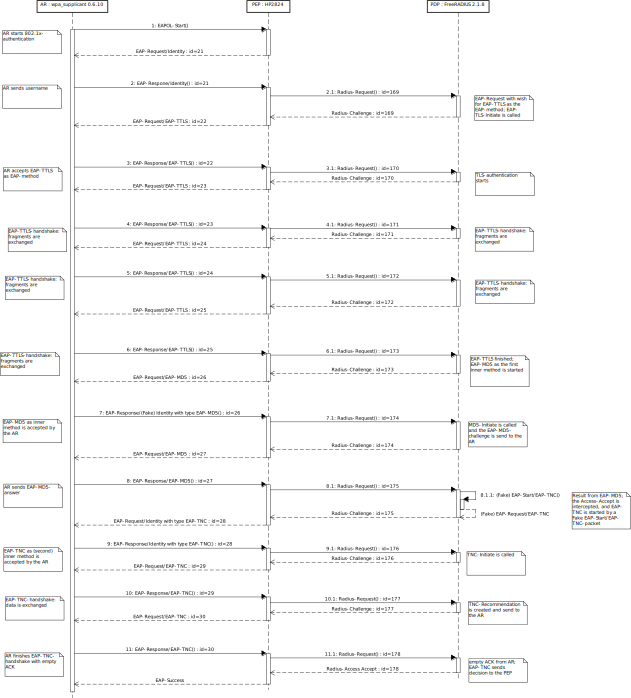
\includegraphics[width=\textwidth]{freeradius-eapttls-patch/diagrams/packet-flow-complete.png}
% 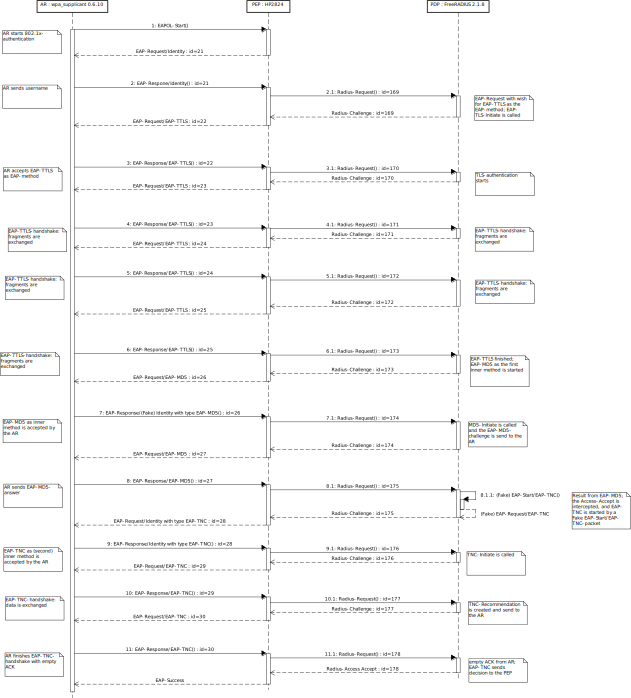
\includegraphics[width=\textwidth]{freeradius-eapttls-patch/diagrams/packet-flow-complete.pdf}
 \caption{EAP TTLS patch packet flow}
 \label{fig:eapttls-patch-flow-1}
\end{figure}

\subsubsection*{Remarks}
The (fake) EAP-Response/Identity of the AR in the EAP-packet with ID 26 is created by wpa\_supplicant.
As a response to the end of the TLS-authentication, a fake EAP-Request/Identity is created inside of wpa\_supplicant,
to start the inner method.
The following debug-output is from wpa\_supplicant, showing this behaviour.

\begin{lstlisting}[style=eapttls-config]
EAP: Received EAP-Request id=26 method=21 vendor=0 vendorMethod=0
...
EAP-TTLS: TLS done, proceed to Phase 2
EAP-TTLS: Derived key - hexdump(len=64): [REMOVED]
EAP-TTLS: received 0 bytes encrypted data for Phase 2
EAP-TTLS: empty data in beginning of Phase 2 - use fake EAP-Request Identity
EAP-TTLS: Phase 2 EAP Request: type=1
EAP: using real identity - hexdump_ascii(len=7):
     74 6e 63 75 73 65 72                              tncuser
EAP-TTLS: AVP encapsulate EAP Response - hexdump(len=12): 02 00 00 0c 01 74 6e 63 75 73 65 72
\end{lstlisting}

\clearpage
\subsection{Configuration}
This chapter describes the configuration of FreeRADIUS and wpa\_supplicant for the use of multiple inner authentication methods.

\subsubsection*{FreeRADIUS}
\paragraph{/usr/local/etc/raddb/users}
The users-file has to contain an entry for a user with a password, so that a user-authentication can take place (EAP-MD5 for example).
\begin{lstlisting}[style=eapttls-config]
# User-entry for EAP-MD5
tncuser Cleartext-Password := password
\end{lstlisting}

\paragraph{/usr/local/etc/raddb/eap.conf}
In the configuration of the EAP-module, several things are important.
The default EAP-type has to be TTLS, and there MUST NOT be a configured instance of EAP-TNC.
This allows a seperation of the incoming requests, as EAP-TNC-packets are only allowed as the second inner method,
and are NOT allowed as the first inner method.
Another important setting is the configuration of the virtual-servers for the EAP-TTLS-module.
At the end, a second instance of the EAP-module has to be configured, with EAP-TNC as the default EAP-type and a configured EAP-TNC-module.
\begin{lstlisting}[style=eapttls-config]
eap {
  # ...
  default_eap_type = ttls
  # ...

  # Comment out the section for TNC
  # tnc {
  # }

  # ...

  ttls {
    default_eap_type = md5
    # ...
    use_tunneled_reply = yes
    #
    virtual_server = "inner-tunnel"
    tnc_virtual_server = "inner-tunnel-second"
  }

  # ...
}

eap eap_tnc {
  default_eap_type = tnc

  tnc {
  }

}
\end{lstlisting}

\paragraph{/usr/local/etc/raddb/sites-enabled/inner-tunnel}
The configuration of the inner tunnel has to be the same as the default-one delivered with FreeRADIUS.

\paragraph{/usr/local/etc/raddb/sites-enabled/inner-tunnel-second}
This virtual server handles the EAP-TNC-packets of the second inner authentication method.
Important is the usage of the second EAP-module instance (eap\_tnc) in the \textit{authorize} and \textit{authenticate}-section.
In the \textit{post-auth}-section the content is the same as in the default configuration for EAP-TNC, when used as the only inner authenticaton method.

\begin{lstlisting}[style=eapttls-config]
# -*- text -*-
######################################################################
#
#	This is a virtual server that handles *only* EAP-TNC
#	requests.
#
#	$Id$
#
######################################################################

server inner-tunnel-second {

  #  Authorization. First preprocess (hints and huntgroups files),
  #  then realms, and finally look in the "users" file.
  #
  #  The order of the realm modules will determine the order that
  #  we try to find a matching realm.
  #
  #  Make *sure* that 'preprocess' comes before any realm if you
  #  need to setup hints for the remote radius server
  authorize {
  #
  #  The preprocess module takes care of sanitizing some bizarre
  #  attributes in the request, and turning them into attributes
  #  which are more standard.
  #
  #  It takes care of processing the 'raddb/hints' and the
  #  'raddb/huntgroups' files.
  #
  #  It also adds the {Client-IP-Address} attribute to the request.
  preprocess

  eap_tnc {
    ok = return
  }
}

#  Authentication.
#
#
#  This section lists which modules are available for authentication.
#  Note that it does NOT mean 'try each module in order'.  It means
#  that a module from the 'authorize' section adds a configuration
#  attribute 'Auth-Type := FOO'.  That authentication type is then
#  used to pick the apropriate module from the list below.
# 

#  In general, you SHOULD NOT set the Auth-Type attribute.  The server
#  will figure it out on its own, and will do the right thing.  The
#  most common side effect of erroneously setting the Auth-Type
#  attribute is that one authentication method will work, but the
#  others will not.
#
#  The common reasons to set the Auth-Type attribute by hand
#  is to either forcibly reject the user, or forcibly accept him.
#
authenticate {
  #
  #  Allow EAP-TNC authentication.
    eap_tnc
}

#  Session database, used for checking Simultaneous-Use. Either the radutmp 
#  or rlm_sql module can handle this.
#  The rlm_sql module is *much* faster
session { 
  radutmp
}

#  Post-Authentication
#  Once we KNOW that the user has been authenticated, there are
#  additional steps we can take.
post-auth {
  if (control:TNC-Status == "Access") {
    update reply {
      Tunnel-Type := VLAN
      Tunnel-Medium-Type := IEEE-802
      Tunnel-Private-Group-ID := 96
    }
  }
  elsif (control:TNC-Status == "Isolate") {
    update reply {
      Tunnel-Type := VLAN
      Tunnel-Medium-Type := IEEE-802
      Tunnel-Private-Group-ID := 97
    }
  }

# Note that we do NOT assign IP addresses here.
# If you try to assign IP addresses for EAP authentication types,
# it WILL NOT WORK.  You MUST use DHCP.
#
#  Access-Reject packets are sent through the REJECT sub-section of the
#  post-auth section.
#
#  Add the ldap module name (or instance) if you have set 
#  'edir_account_policy_check = yes' in the ldap module configuration
#
  Post-Auth-Type REJECT {
    attr_filter.access_reject 
  }
}

} # inner-tunnel-second block
\end{lstlisting}

\subsubsection*{wpa\_supplicant.conf}
The identity and password have to be the same as in the users-configuration on FreeRADIUS.
\begin{lstlisting}[style=eapttls-config]
network={
  ssid="eap_ttls"
  key_mgmt=IEEE8021X
  eap=TTLS
  identity="tncuser"
  password="password"
  ca_cert="/home/tncuser/tnc/certs/ca.pem"
  id_str=""
}
\end{lstlisting}


% ==============================================================================
\section{naaeap}
\subsection{General Information}
The naaeap library processes the TNC specific data that was extracted out of the
EAP-TNC packet by the EAP-TNC module of FreeRADIUS / forwards TNC data for encapsulation
within EAP to that module. The main purpose of naaeap is to handle fragmentation
and establish the communication context to the tncs module.

\subsection{Architecture}
naaeap is provided as shared library. The classes contained are basically separated into
classes providing logic and into classes providing simple entities. Since naaeap
is used by the EAP-TNC module (which is written in C), naaeap exposes a C interface
defined in \texttt{naaeap.h}. The interface includes functions for initialization, connection
management and the processing of TNC data. Most of the calls (except those
that deal with Fragmentation) are forwarded to the tncs module.

\begin{figure}
 \centering
 \includegraphics[width=\textwidth]{design/tncfhh-class-sequence-diagrams-0-6-0/nal-class-0-6-0-light.png}
 \caption{naaeap class diagram (overview)}
 \label{fig:naaeap-overview}
\end{figure}


% ==============================================================================
\section{tncs}
\subsection{General Information}
The tncs receives incoming TNCCS and IMCIMV messages. TNCCS messages
(like preferred language) are directly processed by the tncs. IMCIMV messages are
forwarded to the corresponding IMVs. Routing is based upon the respective message
types. The tncs is responsible for correctly loading/initializing/calling and
terminating all IMVs (those that are specified in the tnc\_config file). Currently,
tncs supports only IF-TNCCS 1.1. Approaches to integrate IF-TNCCS-SoH have not
been finished yet.

\subsection{Architecture}
The TNC server implementation of TNC@FHH. Exposes a C++ interface that is used
by naaeap. The C++ interface is defined in \texttt{Coordinator.h}. It includes
only few methods. The most important ones deal with initialization, connection management
and the processing of TNC data.

\begin{figure}
 \centering
 \includegraphics[width=\textwidth]{design/tncfhh-class-sequence-diagrams-0-6-0/iel-class-0-6-0-light.png}
 \caption{tncs class diagram (overview)}
 \label{fig:tncs-overview}
\end{figure}

\section{imunit}
\subsection{General Information}
imunit provides an easy to use framework for the development of new IMC/IMV
pairs. imunit compiles and runs on many Unix-like systems. Windows is currently
not supported. However, we assume that Windows-support would need only minor
modifications of the build process.\footnote{Appropriate patches are very
welcome ...}

The following TNC interfaces are supported by imunit
\begin{itemize}
 \item IF-IMC 1.2 (\url{http://www.trustedcomputinggroup.org/resources/tnc_ifimc_specification})
 \item IF-IMV 1.2 (\url{http://www.trustedcomputinggroup.org/resources/tnc_ifimV_specification})
\end{itemize}

To demonstrate the use of imunit for the development of new IMC/V pairs, TNC@FHH
contains a very basic exampleimc/v pair.

\subsection{Architecture}
Figure \ref{fig:imunit-overview} gives an overview of the imunit package. The components and
their functions will be described in the following.
\begin{figure}
 \centering
 \includegraphics[width=\textwidth]{design/tncfhh-class-sequence-diagrams-0-6-0/iml-class-0-6-0-light.png}
 \caption{imunit class diagram (overview)}
 \label{fig:imunit-overview}
\end{figure}

On Unix-like Systems, IMCs and IMVs are provided as shared objects (\verb+*.so+). The IMC/V modules
can be used via the IF-IMC/V interface. These interfaces are specified as C-functions. However, the imunit
package is mostly written in C++, allowing us to use an object-oriented design internally.

Besides the C/C++ mapping, there is another interesting issue regarding the instantiation of objects:
in imunit, there is one class that represents the shared library itself (named IMCLibrary/IMVLibrary). Normally,
for a specific IMC or IMV shared library, there will be one object of this class for each TNCC/TNCS running on a platform.

To address the issue that
a TNCC/TNCS can handle multiple connections in parallel, there needs to be a connection-based representation of an IMC/IMV.
This representation is provided by the AbstractIMC/AbstractIMV class. Normally, there will be one object of this class
for each connection that is handled by a TNCC/TNCS on a platform. As a developer of an IMC/V pair, you have to provide your
own implementation of IMCLibrary and AbstractIMC or IMVLibrary and AbstractIMV by inhereting from the classes of the imunit package. The good
thing is that you do not have to deal with plain C this way.

In the following, we will give a short description of each class available in the imunit package. How they can be used to develop
a simple ExampleIMC/V will be discussed in section \ref{sec:example-imcv}.

\subsection{General Classes}
\paragraph{IMUnitLibrary} This class encapsulates the similarities of an IMC and an IMV library. There is exactly one instance of this class
for each TNCC or TNCS that uses the corresponding IMC or IMV library. The main purpose of this class is to provide general information about the
library (name, message types used) and to handle the (de)initialization process. Direct known subclasses are IMCLibrary and IMVLibrary.

\paragraph{AbstractIMUnit} This class encapsulates the similarities of an IMC and an IMV instance that is bound to a specific connection. The connection
is handled via the TNCC or the TNCS. There is normally one instance of this class for each ongoing connection. The class implements methods
that are available for IMCs and for IMVs (notifyConnectionChange(), batchEnding() and receiveMessage()). Direct known subclasses are AbstractIMC
and AbstractIMV.

\paragraph{ResultException}
A simple exception class. Extends \verb+std::exception+. This class can carry a \verb+TNC_Result+ return value. Exceptions of this class
are used internally in the imunit package to handle errors in a more convenient way than it is possible with simple return values. If a TNCC/TNCS
must be notified about an error, the ResultException can be easily mapped to a simple \verb+TNC_Result+ value that is return by an interface C-function.
This class has no known subclasses.

\subsection{IMC-specific Classes}
\paragraph{IMCLibrary}
This class inherits from IMUnitLibrary and encapsulates all IMC specific functionalities of an IMC library. This class multiplexes incoming calls
from an TNCC to a conrete instance of AbstractIMC. Furthermore, it holds all pointers to the TNCC functions as specified by IF-IMC. IMC developers
must extend this class to implement their own IMC library. IMCLibrary defines a pure virtual factory method (createNewImcInstance()) that must
be implemented by the IMC developer.

\paragraph{AbstractIMC}
This class inherits from AbstractIMUnit. It represents instances of an IMC that are bound to a certain connection. It manages the state
of a concrete IMC related to a given connection ID. IMC developers must extend this class to implement their own IMC.
This class defines a pure virtual method (beginHandshake()) that must be implemented by the IMC developer.

\paragraph{TNCC}
This is an interface class that encapsulates all TNCC functions of the IF-IMC interface. It allows AbstractIMC (and the sub-classes implemented
by an IMC developer) to call the TNCC via an instance of this class (instead of directly using C-function pointers). TNCC has no known sub-classes.

\paragraph{IFIMCImpl.cpp (deprecated)}
This "`class"' is actually no class. It contains the mapping from C to C++ for the IMC functions
of IF-IMC. \emph{Note:} This file is empty since version 0.6.0. Its content has been moved to the \verb+TNCFHH_IMCLIBRARY_INITIALIZE+ macro
in IMCLibrary.h. The file will be removed from imunit in the next release.

\subsection{IMV-specific Classes}
\paragraph{IMVLibrary}
This class inherits from IMUnitLibrary and encapsulates all IMV specific functionalities of an IMV library. This class multiplexes incoming calls
from an TNCS to a conrete instance of AbstractIMV. Furthermore, it holds all pointers to the TNCS functions as specified by IF-IMV. IMV developers
must extend this class to implement their own IMV library. IMVLibrary defines a pure virtual factory method (createNewImvInstance()) that must
be implemented by the IMV developer.

\paragraph{AbstractIMV}
This class inherits from AbstractIMUnit. It represents instances of an IMV that are bound to a certain connection. It manages the state
of a concrete IMV related to a given connection ID. IMV developers must extend this class to implement their own IMV.

\paragraph{TNCS}
This is an interface class that encapsulates all TNCS functions of the IF-IMV interface. It allows AbstractIMV (and the sub-classes implemented
by an IMV developer) to call the TNCS via an instance of this class (instead of directly using C-function pointers). TNCS has no known sub-classes.

\paragraph{IFIMVImpl.cpp (deprecated)}
This "`class"' is actually no class. It contains the mapping from C to C++ for the IMV functions
of IF-IMV. \emph{Note:} This file is empty since version 0.6.0. Its content has been moved to the \verb+TNCFHH_IMVLIBRARY_INITIALIZE+ macro
in IMVLibrary.h. The file will be removed from imunit in the next release.

% ==============================================================================
\section{IMC/V Pairs}
\subsection{TNC@FHH IMC/V Pairs Message Types}\label{sec:message-types}
TNC@FHH IMC/V pairs use the following message types:
\begin{itemize}
	\item vendord id (FHH IANA PEN): 0x0080ab
	\item example: 0xfe
	\item dummy: 0x31
	\item clamav: 0x41
	\item platid: 0x33
	\item attestation: 0x34
	\item hostscanner: 0x30
\end{itemize}

\subsection{example}\label{sec:example-imcv}
\subsubsection{General Information}
This is a helloworld example for an IMC/V that is implemented based upon imunit.
In the remainder of this section, a step-by-step guide that explains how to implement
your own IMC/V based upon imunit is given.

\subsubsection{Architecture}
The architecture of the exampleimc/v is very simple. There are just four classes
for both the IMC and the IMV:
\begin{itemize}
	\item ExampleIMCLibrary
	\item ExampleIMC
	\item ExampleIMVLibrary
	\item ExampleIMV
\end{itemize}
Each class extends the corresponding imunit class. There are no external files,
processes or programs used by the exampleimc/v.

\subsubsection{Coding the exampleimc}
\begin{enumerate}
 \item Create a class ExampleIMCLibrary that extends IMCLibrary.
 \begin{enumerate}
  \item Define the message types for your IMC. Normally, each IMC has its own message type\footnote{This
  will likely change when IF-M is released.} (done in ExampleIMCLibrary.h). The message type is used for two purposes: 1) it is used
  to indicate the type of messages send to the TNCC and 2) it is used to tell the TNCC which message types the IMC is interested in receiving.
  \begin{lstlisting}
  /* define Vendor ID (see IANA PEN). */
  #define VENDOR_ID 0x0080ab
  /* define Messagesubtype */
  #define MESSAGE_SUBTYPE 0xfe
  \end{lstlisting}

  \item Implement a ctor (and dtor if necessary). Add your message type defined above to the list
  of message types the IMC wants to receive.
  \begin{lstlisting}
  ExampleIMCLibrary::ExampleIMCLibrary()
  {
    LOG4CXX_INFO(logger, "Load ExampleIMC library ");
    /* set all attributes inherited from tncfhh::iml::IMCLibrary */
    // the library name for logging
    this->imUnitLibraryName = "ExampleIMC";
    // add an messageType composed of Vendor ID (IANA PEN) and MessageSubtype
    this->addMessageType(VENDOR_ID, MESSAGE_SUBTYPE);
  }
  \end{lstlisting}

  \item Initialize the imunit framework (done in ExampleLibrary.cpp). This defines
  the C-functions interface according to IF-IMC and maps those functions to C++ methods
  of imunit. You must provide the class name of your ExampleIMCLibrary implementation
  as argument. This causes the framework to create an instance of ExampleIMCLibrary
  within the initialization macro.
  \begin{lstlisting}
  // TNC@FHH IMCLibrary Initialization +
  // implement IF-IMC c-functions
  TNCFHH_IMCLIBRARY_INITIALIZE(ExampleIMCLibrary) ;
  \end{lstlisting}

  \item Implement the pure virtual factory method. This method creates a new instance of
  the ExampleIMC class (described in step 2). The method is called when a new connection
  is created. The memory is freed when the same connection is deleted.
  \begin{lstlisting}
  tncfhh::iml::AbstractIMC *ExampleIMCLibrary::createNewImcInstance(TNC_ConnectionID conID)
  {
    LOG4CXX_TRACE(logger, "createNewImcInstance( " << conID << ")");
    // just return a new instance of ExampleIMC
    return new ExampleIMC(conID, this);
  }
  \end{lstlisting}
 \end{enumerate}

 \item Create a class ExampleIMC that extends AbstractIMC.
 \begin{enumerate}
  \item Define the ctor (and dtor if necessary). The ctor needs the connection ID and a pointer to the
  corresponding ExampleIMCLibrary as arguments. Internally, this causes the instantiation of a TNCC object
  which can forward the calls to the ``real'' TNCC via the pointer to the ExampleIMCLibrary (which holds the
  function pointers to the ``real'' TNCC). The benefit is: you as IMC developer can call methods of the TNCC
  instantiation to talk to the ``real'' TNCC.
  \begin{lstlisting}
  ExampleIMC::ExampleIMC(TNC_ConnectionID conID, ExampleIMCLibrary *pExampleIMCLibrary)
    :AbstractIMC(conID, pExampleIMCLibrary)
  {
    // initialize
  }
  \end{lstlisting}

  \item Implement the (pure virtual) mandatory beginHandshake() method. In this case, our IMC sends a first message
  to its ExampleIMV (by calling sendMessage() of the TNCC).
  \begin{lstlisting}
  TNC_Result ExampleIMC::beginHandshake()
  {
    LOG4CXX_TRACE(logger, "beginHandshake()");
    // this message should be send to ExampleIMV
    std::string sendMessage("Example message from ExampleIMC");
    LOG4CXX_TRACE(logger, "Send Message: " << sendMessage);
    // send message
    this->tncc.sendMessage((unsigned char*)sendMessage.c_str(), sendMessage.size()+1/*for'\0'*/, VENDOR_ID, MESSAGE_SUBTYPE);
    // return all ok
    return TNC_RESULT_SUCCESS;
  }
  \end{lstlisting}

  \item Implement optional methods. These are already implemented by the imunit
  framework. But normally, to have them behave in a reasonable (from the IMC developers point of view) manner,
  these should be overwritten. We will override all optional methods.
  \begin{enumerate}
   \item Implement receiveMessage(). This is called to deliver a message from the IMV which was received by the TNCC to the IMC. Here, our IMC just
   sends another message.
  \begin{lstlisting}
  TNC_Result ExampleIMC::receiveMessage(TNC_BufferReference message, TNC_UInt32 messageLength, TNC_MessageType messageType)
  {
    LOG4CXX_DEBUG(logger, "receiveMessage round " << this->getRound());
    // print received message dirty out. WARNING: don't ape this,
    // message should end with non-null! Heed: Message can be evil!
    LOG4CXX_INFO(logger, "Received Message: " << message);
    // this message should be send to ExampleIMV
    std::string sendMessage("Another example message from ExampleIMC.");
    LOG4CXX_INFO(logger, "Send Message: " << message);
    // send message
    this->tncc.sendMessage((unsigned char*)sendMessage.c_str(), sendMessage.size()+1/*for'\0'*/, VENDOR_ID, MESSAGE_SUBTYPE);
    // return all ok
    return TNC_RESULT_SUCCESS;
  }
  \end{lstlisting}

  \item Implement batchEnding(). Here, it basically does nothing.
  \begin{lstlisting}
  TNC_Result ExampleIMC::batchEnding()
  {
    LOG4CXX_TRACE(logger, "batchEnding");
    // return all ok
    return TNC_RESULT_SUCCESS;
  }
  \end{lstlisting}

  \item Implement notifyConnectionChange(). The new connection state can be queried via the getConnectionState() method.
  Here, it basically does nothing. Normally, you would change the state of your IMC according to the connection state.
  \begin{lstlisting}
  TNC_Result ExampleIMC::notifyConnectionChange()
  {
    LOG4CXX_TRACE(logger, "notifyConnectionChange");
    /* if new handshake start */
    if(this->getConnectionState() == TNC_CONNECTION_STATE_HANDSHAKE)
    /* reset IMC */;
    // return all ok
    return TNC_RESULT_SUCCESS;
  }
  \end{lstlisting}

  \end{enumerate}

 \end{enumerate}
 \item Finished. Thats all for the IMC part.
\end{enumerate}

\subsubsection{Coding the exampleimv}
Coding the ExampleIMV conceptually works the same as coding the ExampleIMC. There are only minor differences
regarding which methods must be overwritten/implemented.
\begin{enumerate}
 \item Create a class ExampleIMVLibrary that extends IMVLibrary.
 \begin{enumerate}
  \item Define the message types for your IMV. Normally, each IMV has its own message type\footnote{This
  will likely change when IF-M is released.} (done in ExampleIMVLibrary.h). The message type is used for two purposes: 1) it is used
  to indicate the type of messages send to the TNCS and 2) it is used to tell the TNCS which message types the IMV is interested in receiving.
  \begin{lstlisting}
  /* define Vendor ID (see IANA PEN). */
  #define VENDOR_ID 0x0080ab
  /* define Messagesubtype */
  #define MESSAGE_SUBTYPE 0xfe
  \end{lstlisting}

  \item Implement a ctor (and dtor if necessary).  Add your message type defined above to the list
  of message types the IMV wants to receive.
  \begin{lstlisting}
  ExampleIMVLibrary::ExampleIMVLibrary()
  {
    LOG4CXX_INFO(logger, "Load ExampleIMV library ");
    /* set all attributes inherited from tncfhh::iml::IMVLibrary */
    // the library name for logging
    this->imUnitLibraryName = "ExampleIMV";
    // add an messageType composed of Vendor ID (IANA PEN) and MessageSubtype
    this->addMessageType(VENDOR_ID, MESSAGE_SUBTYPE);
  }
  \end{lstlisting}

  \item Initialize the imunit framework (done in ExampleIMVLibrary.cpp). This defines
  the C-functions interface according to IF-IMV and maps those functions to C++ methods
  of imunit. You must provide the class name of your ExampleIMVLibrary implementation
  as argument. This causes the framework to create an instance of ExampleIMVLibrary
  within the initialization macro.
  \begin{lstlisting}
  // TNC@FHH IMVLibrary Initialization +
  // implement IF-IMV c-functions
  TNCFHH_IMVLIBRARY_INITIALIZE(ExampleIMVLibrary) ;
  \end{lstlisting}

  \item Implement the pure virtual factory method. This method creates a new instance of
  the ExampleIMV class (described in step 2). The method is called when a new connection
  is created. The memory is freed when the same connection is deleted.
  \begin{lstlisting}
  tncfhh::iml::AbstractIMV *ExampleIMVLibrary::createNewImvInstance(TNC_ConnectionID conID)
  {
    LOG4CXX_TRACE(logger, "createNewImvInstance( " << conID << ")");
    // just return a new instance of ExampleIMV
    return new ExampleIMV(conID, this);
  }
  \end{lstlisting}
 \end{enumerate}

 \item Create a class ExampleIMV that extends AbstractIMV.
 \begin{enumerate}
  \item Define the ctor (and dtor if necessary). The ctor needs the connection ID and a pointer to the
  corresponding ExampleIMVLibrary as arguments. Internally, this causes the instantiation of a TNCS object
  which can forward the calls to the ``real'' TNCS via the pointer to the ExampleIMVLibrary (which holds the
  function pointers to the ``real'' TNCS). The benefit is: you as IMV developer can call methods of the TNCS
  instantiation to talk to the ``real'' TNCS.
  \begin{lstlisting}
  ExampleIMV::ExampleIMV(TNC_ConnectionID conID, ExampleIMVLibrary *pExampleIMVLibrary)
    :AbstractIMV(conID, pExampleIMVLibrary)
  {
    // initialize
  }
  \end{lstlisting}

  \item In contrast to the IMC part, there is no mandatory (pure virtual) method that must be implemented by ExampleIMV. However, we will
  override several optional methods.

  \begin{enumerate}
   \item Implement receiveMessage(). This is called to deliver a message from the IMC which was received by the TNCS to the IMV. Here, our IMV sends a new message
   if this is the first round of the TNC handshake. Otherwise, it provides an allow recommendation. The round counter is managed by the imunit
   framework as follows:
   \begin{itemize}
    \item set to 0 at the end of IMC/VLibrary::notifyConnectionChange() when called with newState == \verb+TNC_CONNECTION_STATE_HANDSHAKE+
    \item for IMC/V  : increased before IMC/VLibrary::batchEnding returns
    \item for the IMC: increased before IMCLibrary::beginHandshake returns
   \end{itemize}
  \begin{lstlisting}
TNC_Result ExampleIMV::receiveMessage(TNC_BufferReference message, TNC_UInt32 messageLength, TNC_MessageType messageType)
{
  LOG4CXX_DEBUG(logger, "receiveMessage round " << this->getRound());
  // print received message dirty out. WARNING: don't ape this,
  // message should end with non-null! Heed: Message can be evil!
  LOG4CXX_INFO(logger, "Received Message: " << message);
  /* only send one message to ExampleIMC */
  if (this->getRound() < 1) {
    // this message should be send to ExampleIMC
    std::string sendMessage("Example message from ExampleIMV");
    LOG4CXX_INFO(logger, "Send Message: " << sendMessage);
    // send message
    this->tncs.sendMessage((unsigned char*)sendMessage.c_str(), sendMessage.size()+1/*for'\0'*/, VENDOR_ID, MESSAGE_SUBTYPE);
  } else {
    /* validation finish, set recommendation & co */
    validationFinished = true;
    // for access allow:
    actionRecommendation = TNC_IMV_ACTION_RECOMMENDATION_ALLOW;
    // set evaluation (see TNC_IMV_EVALUATION_RESULT_...)
    evaluationResult = TNC_IMV_EVALUATION_RESULT_DONT_KNOW;
  }
  // return all ok
  return TNC_RESULT_SUCCESS;
}
  \end{lstlisting}

  \item Implement batchEnding(). Here, it basically does nothing.
  \begin{lstlisting}
  TNC_Result ExampleIMV::batchEnding()
  {
    LOG4CXX_TRACE(logger, "batchEnding");
    // return all ok
    return TNC_RESULT_SUCCESS;
  }
  \end{lstlisting}

  \item Implement notifyConnectionChange(). The new connection state can be queried via the getConnectionState() method.
  Here, it basically does nothing. Normally, you would change the state of your IMV according to the connection state.
  \begin{lstlisting}
  TNC_Result ExampleIMV::notifyConnectionChange()
  {
    LOG4CXX_TRACE(logger, "notifyConnectionChange");
    /* if new handshake start */
    if(this->getConnectionState() == TNC_CONNECTION_STATE_HANDSHAKE)
    /* reset IMV */;
    // return all ok
    return TNC_RESULT_SUCCESS;
  }
  \end{lstlisting}

  \end{enumerate}

 \end{enumerate}
 \item Finished. Thats all for the IMV part.
\end{enumerate}

\subsection{dummy}
\subsubsection{General Information}
This is another helloworld example for an IMC/V that is implemented based upon imunit.
The IMC reads a local file, sends the content to the IMV, which provides
a recommendation based upon this message.

\subsubsection{Architecture}
The architecture of the dummyimc/v is very simple. The IMC sends the content of a local
file to the IMV. The content is either "allow", "isolate", or "none", that correspond
to the respective TNC recommendations. The default location of the policy is
\texttt{/etc/tnc/dummyimc.file}. The IMV uses a policy that defines how many
messages it wants to receive before a recommendation is granted. The default
location of the policy is \texttt{/etc/tnc/dummyimv.policy}.

\subsection{clamav}
\subsubsection{General Information}
The clamav IMC/V checks the status of the anti virus software ClamAV. The IMC/V pair
supports the evaluation of the following properties:
\begin{itemize}
	\item Operational Status of clamd
	\item Version of clamav
	\item Version of main
	\item Version of daily
\end{itemize}
The baseline for this evaluation is the clamavimv.policy file. This is a simple
text file that enables you to specify the desired good values of an endpoint's
ClamAV configuration. The file is commented extensively. The policy file is
read at the beginning of each new handshake. Remediation is not supported in
this version. If the data received from the clamavimc matches the desired values
in the policy, an 'ALLOW' recommendation is provided. Otherwise, an 'ISOLATE'
recommendation is provided.

\subsubsection{Architecture}
The IMC/V pair consists of four classes that extend those of the imunit framework (like
the exampleimc/v from section \ref{sec:example-imcv}). In order to work properly,
the clamavimc needs a configuration file. The default location is
\texttt{/etc/tnc/clamavimc.conf}. The file is commented extensively. The clamavimv
needs a policy file where the desired, reference values are specified. The default
location of the policy is \texttt{/etc/tnc/clamavimv.policy}. The file is commented
extensively. The measurement values on the AR are obtained by using the clamconf
utility of Clamav. Depending on last clamav update (full or incremental) the filname 
ending for main and daily can be *.cvd or *.cld. Former versions to 0.7.0 of clamavimc/v
did not consider this. 

\subsection{platid}
\subsubsection{General Information}
The idea of this IMC/V pair is to enable interoperable platform identification.
It implements a simple challenge/response protocol. The IMC signs the challenge
with its RSA private key. The IMV validates if the signature obtained from the
IMC is good and if the corresponding public key has been properly registered (e.g.
whether it is a known platform or not). The key management is based upon
X.509 certificates. As a special feature, the IMC supports to use a TPM protected
key. The openssl\_tpm\_engine package from the TrouSerS project is needed to accomplish
this.

The protocol is as follows: The IMV receives a complete X.509 certificate
from the IMC. The IMV then sends back a random nonce to the IMC which is encrypted
with the RSA private key. The IMV decrypts the encrypted nonce with the public key
contained in the X.509 certificate and compares it with the one which was
send. Additionally the IMV compares the issuername and fingerprint of the
X.509 certificate with entries configured in its policy.

\subsubsection{Architecture}
The IMC is configured via a file. The default location is \texttt{/etc/tnc/platidimc.file}
It cotains information for the IMC where to find the platform's X.509 certificate
and the corresponding RSA private key. The default location of the IMV policy is
\texttt{/etc/tnc/platidimv.certs}.

The IMC/V pair uses open\_ssl for cryptographic operations. If a TPM based key
should be used, the IMC additionally needs TrouSerS and the openssl\_tpm\_engine.
Please refer to the TrouSerS documentation for information how to set up the TPM engine. 

\subsection{attestation}
\subsubsection{General Information} 
The attestation IMC/V pair implements a simple protocol for binary attestation. The integrity
of the AR is verified based on its TPM PCR values.

The following steps give a brief overview of the imc/v handshake:
\begin{itemize}
	\item{Step 1: IMC sends its AIK X.509 certificate.}
	\item{Step 2: IMV verifies AIK certificate.}
	\item{Step 3: IMV sends PCR\_SELECTION to IMC.}
	\item{Step 4: IMC generates TPM Quote based on PCR\_SELECTION and sends it back to IMV.}
	\item{Step 5: IMV generates separate TPM Quote based on PCR reference values.}
	\item{Step 6: IMV compares own TPM Quote with IMC TPM Quote and verifies IMC TPM Quote signature.}
	\item{Step 7: According to operation mode, step 3-6 can be repeated several times.}
	\item{Step 8: Depending on validation in step 6, IMV provides "ALLOW" or "NO\_ACTION" recommendation.}
\end{itemize}

TPM PCR values are SHA-1 hashes which represent available hard- and software on a computer system, as well as the configuration thereof. These values are usually determined during system start (trusted boot).
TrustedGRUB extends the open-source bootloader GNU GRUB with TPM support
to measure the binary configuration (i.e., the identity) of modules to be loaded.
Further information can be found at \url{http://sourceforge.net/projects/trustedgrub/}.
Therefore a working TPM is needed as well as a Trusted Software Stack (TSS) for TPM access, e.g. TrouSerS.

Attestation Identity Keys (AIKs) are used to ensure that PCR values (a TPM Quote) come from a trustworthy TPM.
Due to the fact that current version of attestationIMC/V is not capable of verifying a CA certificate path, a fingerprint of all used AIK credentials must be made known to the IMV.

\subsubsection{Architecture}

IMV policy is located at \code{/etc/tnc/attestationimv.policy} and contains
a list of PCRs with their associated, desired reference values.
Two modes of operation are available. \code{quoteType=single} requests PCRs sequentially one after another.
\code{quoteType=complete} asks the IMC to quote all given PCRs at once.
Single quote mode allows you to determine which PCR value does not match the policy but also causes 
one batch per PCR value, resulting in a higher amount of network traffic.
The TPM Quote is basically a SHA-1 hash of the TCPA\_QUOTE\_INFO structure.
TPM quoting request is performed by the corresponding calls to the TSS,
e.g. TrouSerS since version 0.3.4 is needed.
This version of attestationIMV does not support different policies (PCR values) per AR.
To prevent replay attacks a random 20 byte nonce is also part of each PCR\_SELECTION.

IMC configuration is located at \code{/etc/tnc/platidIMC.file} and contains a path to the 
X509 certificate and its corresponding private-key (AIK).
Currently, tools from \url{http://www.privacyca.com} are used
to create AIKs. The code from \code{identity.c} creates a AIK
blob and a corresponding X.509 certificate.
The SHA-1 hash from this certificate can be extracted by using
 \code{x509} tool from OpenSSL.

\subsection{hostscanner}
\subsubsection{General Information}
The hostscannerimc/v scans for opened ports on an endpoint. The ports to be scanned and 
the expected status of these ports are defined in the IMVs policy file.

\subsubsection{Architecture}
In the IMV's policy, a list of ports with their desired status can be specified.
The default location of the policy is \texttt{/etc/tnc/hostscannerimv.policy}.
The IMC does not require a configuration file.


\section{tncsim}
\subsection{General Information}
tncsim is a simple program that allows you to test IMC/V pairs locally on one
endpoint. tncsim loads IMCs and IMVs and initiates a single TNC handshake. Lots
of debug information is printed out, including the binary structure of the TNC
packets sent from TNCC to TNCS and vice versa.

\subsection{Architecture}
In its default configuration, tncsim uses libtnc as client and TNC@FHH tncs
as server. IMC/V pairs that shall be loaded are specified in \texttt{/etc/tnc/tncsim\_config}.
tncsim can be extended to support arbitrary TNCC and TNCS implementations. For
details, please refer to the sourcecode.

% ==============================================================================
\section{Copyright and License}
This software is Copyright (C) 2010
Fachhochschule Hannover (University of Applied Sciences and Arts).
Use is subject to license conditions.
The main licensing options available are Open Source or Commercial:

\paragraph{Open Source Licensing} This is the appropriate option if you want to
share the source code of your application with everyone you
distribute it to, and you also want to give them the right to share
who uses it. If you wish to use TNC@FHH under Open Source Licensing,
you must contribute all your source code to the open source
community in accordance with the GPL Version 2 when your application
is distributed. See http://www.gnu.org/copyleft/gpl.html

\paragraph{Commercial Licensing} This is the appropriate option if you are
creating proprietary applications and you are not prepared to
distribute and share the source code of your application.
Contact trust@f4-i.fh-hannover.de for details.

% ==============================================================================
\section{Acknowledgement}
TNC@FHH is implemented by the Trust@FHH research group of the Fachhochschule Hannover, the University of Applied Sciences and Arts, located in Lower Saxony, Germany. Parts of this work have been carried out within the tNAC research project (support code 1704B08) which is funded by the German Federal Ministry of Education and Research (\url{http://www.bmbf.de/en/index.php}).


\end{document}
